\section{Power Systems and Frequency}
Interconnected power systems are comprised of power generating units and energy storage systems connected to transmission and distribution networks. Generated power is used to service load demand. A single line diagram of a power network can be seen in Figure \ref{fig:201_power_system}. The diagram shows how thermal generation units (left-hand side), such as coal and nuclear, in addition to renewable sources of generation, like wind and solar provide a power generation mix that is transmitted by a network for the consumers of generated energy: industry and households (right-hand side).
\begin{figure}[ht]
	\centering
	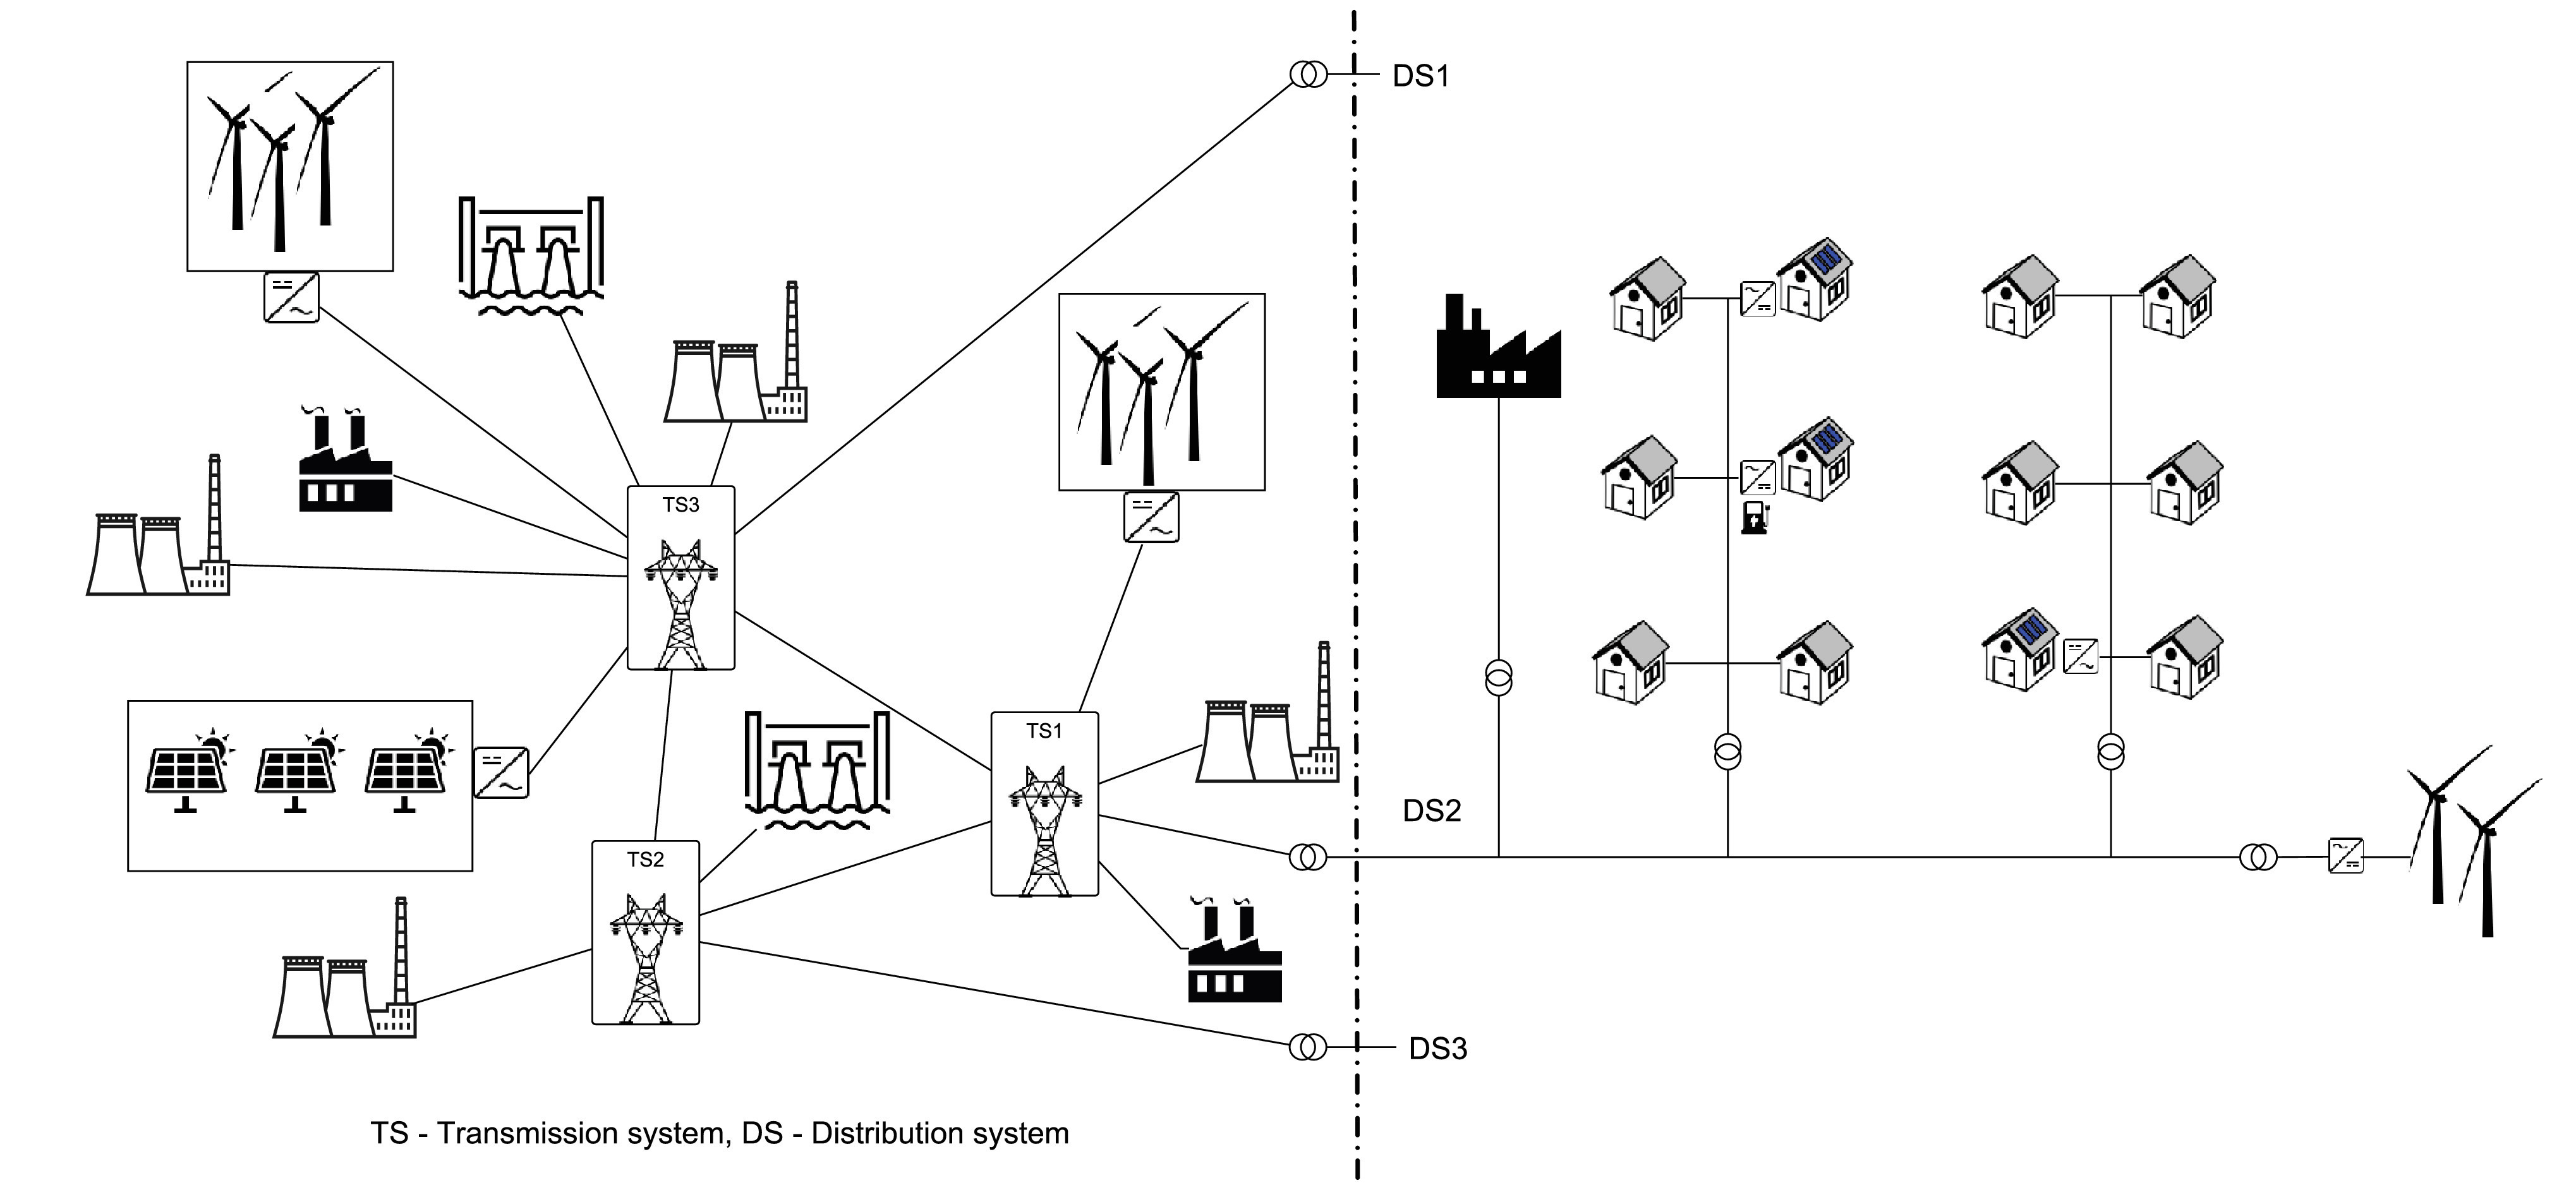
\includegraphics[scale=0.85]{201_power_system}
	\caption[High level overview of a power network]{A single line diagram of a typical power system. The image shows points of generation from thermal and renewable sources, and the subsequent supply of generated energy to meet load demand through the transmission and distribution network \cite{Glavic2019}.}
	\label{fig:201_power_system}
\end{figure}

One of the key elements to successful operation of interconnected power systems is ensuring total load demand is matched with total generation, while taking into account power losses involved with generation, transmission, and distribution \cite{Wood2013}. To understand why it is important to match generation with load demand consider the basic operation of a single thermal generator. 
\begin{figure}[h]
	\centering
	\resizebox{15cm}{!}{\usetikzlibrary{arrows.meta}

\begin{tikzpicture}
	
	
	\draw[rotate=90] (0,5) ellipse (2 and 0.5);
	\draw[rotate=90] (-2,0) arc (180:360:2 and 0.5);
	\draw (-5,-2) -- (0,-2);
	\draw (-5,2) -- (0,2);
	
	\draw[rotate=90] (-1,-5) arc (180:360:1 and 0.25);
	\draw[rotate=90] (-2,-5) arc (180:360:2 and 0.5);
	\draw[rotate=90] (-2,-5) arc (180:240:2 and -0.5);
	\draw[rotate=90] (2,-5) arc (360:300:2 and -0.5);
	\draw[rotate=90] (-2,-12) arc (180:360:2 and 0.5);
			
	\draw[rotate=90] (-1,-0.44) -- (-1,-5);
	\draw[rotate=90] (1,-0.44) -- (1,-5);
	\draw[rotate=90] (-2,-5) -- (-2,-12);
	\draw[rotate=90] (2,-5) -- (2,-12);
	
	\draw[-Latex] (-12,0) -- (-6,0);
	\draw[-Latex] (13,0) -- (19,0);
	
	\draw[rotate=90, -latex, color=magenta, ultra thick] (-2,-2) arc (180:410:2 and 0.8);
	
	\draw[rotate=90, -latex, color=magenta, ultra thick] (3,3) arc (360:200:3 and 1.25);
	
	\node at (-2,-4) {\Large\textbf{TURBINE}};
	\node at (8.5,-4) {\Large\textbf{GENERATOR}};
	
	\node at (-1, -3) {\LARGE$T_{mech}$};
	\node at (3, 2) {\LARGE$T_{elec}$};
	
	\node at (-9,1) {\Large\textbf{Mechanical Energy}};
	\node at (16,1) {\Large\textbf{Electrical Energy}};
		
\end{tikzpicture}
}
	\caption[Turbine generator model]{A thermal generation unit consisting of a prime mover (turbine), and a synchronous machine \cite{Wood2013}.}
	\label{fig:202_generation}
\end{figure}

The essential elements of a thermal generator are a prime mover (such as a gas turbine) and a synchronous machine, as depicted in Figure \ref{fig:202_generation}. The prime mover provides mechanical torque, $T_{mech}$, which drives the synchronous machine producing electrical energy. In response, the synchronous machine creates an opposing torque that depends on the size of the load demand. This opposing torque is referred to as electrical torque and is denoted as $T_{elec}$. If $\alpha$ represents angular acceleration of the generator rotating mass, and $I$ is its moment of inertia, then by Newton's second law:
\begin{equation}
	T_{mech} - T_{elec} = I \alpha. \label{eq:201}
\end{equation}

When $T_{mech}$ equals $T_{elec}$ the system will be in a steady state of zero angular acceleration with a constant angular velocity, $\omega$. Now, if $T_{mech} > T_{elec}$, then the system has an angular acceleration causing the angular velocity, $\omega$, to increase. This results in a frequency increase in the system. Conversely, if $T_{mech} < T_{elec}$ then the angular velocity $\omega$ will decrease, resulting in a frequency decrease. It is important to note that at any point in time, the total electrical load demand will fluctuate as consumers switch grid connected appliances or motors on and off. The result is that an uncontrolled system will have a continually changing frequency. Australia's electricity network is designed to operate at a frequency of 50$\si{\hertz}$. In the majority of network scenarios, the Australian Energy Market Operator (AEMO) has a desired operating range for frequency which lies between 49.85 and 50.15$\si{\hertz}$ \cite{AEMOfreqdev}. Similarly, the Power and Water Corporation (PWC) network technical code for the Northern Territory states that under normal operating conditions frequency should be maintained in the range of 49.80 to 50.20$\si{\hertz}$ \cite{Pwc2013}. Network operation outside of the specified range can cause damage to electrical equipment such as transformers or motors, which are designed to operate at specific frequencies \cite{Sen2014}. Network designers engineer protection schemes so that sustained frequency excursions outside of the allowed range will cause equipment to trip from the network \cite{AEMOpowerfreqriskrev}.

\begin{figure}[ht]
	\centering
	\documentclass{standalone}
\usepackage{tikz}
\usepackage{pgfplots}
\usepgfplotslibrary{dateplot, statistics}

\begin{document}
\begin{tikzpicture}
	\begin{axis}[
		compat=newest,
		no markers,
		tick pos=left,
		width=0.8\textwidth,
		height=0.35\textwidth,
		xlabel=time,
		x label style={at={(axis description cs:0.5,-0.2)},font=\scriptsize},
		xticklabel style={/pgf/number format/1000 sep=,rotate=60,anchor=east,font=\scriptsize},
		ylabel=MW,
		y label style={font=\scriptsize},
		yticklabel style={/pgf/number format/1000 sep=,font=\scriptsize},
		legend pos={north west},
		legend style={font=\scriptsize},
		date coordinates in=x,
		xticklabel=\hour:\minute
	]
	\addplot[green!20!gray, ultra thick] table[mark=none, x=time, y=demand, col sep=comma] {system_demand_data.csv};
	
	\end{axis}
\end{tikzpicture}
\end{document}
	\caption[Intraday load demand profile]{Weekday energy demand profile in South Australia during summer \cite{Aemosaenergyrep}.}
	\label{fig:203_load_profile}
\end{figure}

\newpage

Protection schemes tripping equipment from the network is undesirable as this can leave consumers without power, resulting in economic loss. Further, if disconnections are uncontrolled the system stability is reduced \cite{AEMOpowerfreqriskrev}. System controllers, such as the AEMO and PWC, are interested in being able to control the system to follow changes in load demand so that system frequency is maintained in the allowable range. Additionally, they are interested in control mechanisms to restore frequency excursions as a result of unexpected disturbances. System controllers can use historical data, like that shown in Figure \ref{fig:203_load_profile}, to forecast daily demand profiles with some reliability. This type of forecasting does not help when trying to predict the occurrence of random disturbances; however, it does provide a starting point for estimating required generation needed to meet demand. It is important to note that forecasting is not perfect. Inevitably mismatches in supply and demand will occur causing small imbalances between $T_{mech}$ and $T_{elec}$, resulting in a change to angular velocity $\omega$ and the network frequency \cite{Glover2012}. To perfectly match supply and demand, system controllers use generators referred to as regulating units, placed under Automatic Generation Control (AGC) \cite{Kothari2011}. A regulating unit is a generator that has the capacity to increase or decrease mechanical torque $T_{mech}$, and the AGC is a system providing control over the mechanical torque output of regulating generators. If the system controller has a sufficient number of regulating units under AGC it can perform two functions: load following, and restoring the system to stable operating conditions in the event of a disturbance \cite{Grainger1994}. Using a regulating unit under AGC control to load follow is referred to, by AEMO, as load following ancillary services \cite{AEMOancilliaryserv}.

\begin{figure}[ht]
	\centering
	\documentclass{standalone}
\usepackage{tikz}
\usepackage{pgfplots}

\begin{document}
\begin{tikzpicture}
	\begin{axis}[
		compat=newest,
		no markers,
		tick pos=left,
		width=0.8\textwidth,
		height=0.35\textwidth,
		xlabel=time (sec),
		x label style={at={(axis description cs:0.5,-0.2)},font=\scriptsize},
		xticklabel style={/pgf/number format/1000 sep=,font=\scriptsize},
		ylabel=frequency (Hz),
		y label style={font=\scriptsize},
		yticklabel style={/pgf/number format/1000 sep=,font=\scriptsize},
		legend pos={north west},
		legend style={font=\scriptsize},
		xmin=0, xmax=80,
		ymin=49.55 , ymax=50.10
	]
	\addplot[green!20!gray, smooth] table[mark=none, x=time, y=frequency, col sep=comma] {frequency_disturbance.csv};
	
	\addplot +[mark=none, dashed, black] coordinates {(2, 49.55) (2, 50.10)};
	
	\addplot +[mark=none, dashed, black] coordinates {(20, 49.55) (20, 50.10)};
	
	\addplot +[mark=none, dashed, black] coordinates {(40, 49.55) (40, 50.10)};
	
	\end{axis}
\end{tikzpicture}
\end{document}
	\caption[Frequency profiles of differing disturbance types]{A minor frequency disturbance occurs at the 2 sec mark and primary control systems (governors) arrest the frequency drop. System frequency is adjusted to desired 50$\si{\hertz}$ operating level using AGC control of regulating units. This is referred to as supplementary (or secondary) control. At the 40 sec mark the network experiences a major frequency disturbance which is arrested by emergency control measures such as under-frequency load shedding (UFLS). System restoration is aided using AGC control of regulating units, which AEMO refers to as spinning reserve ancillary services \cite{Bevrani2011}.}
	\label{fig:204_frequency_arrest}
\end{figure}

\newpage

Load following control adjusts regulating units in order to match supply with a demand load profile, and maintain frequency in a normal operating range a shown in the first 40 seconds of Figure \ref{fig:204_frequency_arrest}. Using a regulator under AGC control to restore the system after a major disturbance is referred to, by AEMO, as providing spinning reserve ancillary services. \cite{AEMOancilliaryserv}. When used in either fashion it is important to note that the regulating unit is not responsible for arresting frequency excursions, rather, it is used to restore the system back to the allowable frequency operating range after the frequency excursion has been arrested. An example of a frequency excursion, arrest, and subsequent restoration for minor and major disturbances can be seen in Figure \ref{fig:204_frequency_arrest}. AEMO and PWC do not require all generators on the network to act as regulating units since adequate frequency control can be achieved using a subset of the total available generators.

%------------------------ SS: Modelling a Single Area

\subsection{Modelling a Single Area System}\label{sec:modelling_a_single_area}
The power system model shown in Figure \ref{fig:201_power_system} depicts total generation coming from many generation assets. This is complex to model. Generation assets are often divided into sub-groups referred to as control areas \cite{Kothari2011}. A control area is defined as a subset of generators that are in close proximity to each other and constitute a coherent group that speed up and slow down together, maintaining their relative power angles \cite{Kothari2011}. Therefore, the total network is comprised of many interconnected control areas. An example of this can be seen in Figure \ref{fig:2105_multiple_area_system}. Notice that for each area there is only one load and one generator.
\begin{figure}[ht]
	\centering
	\resizebox{12cm}{!}{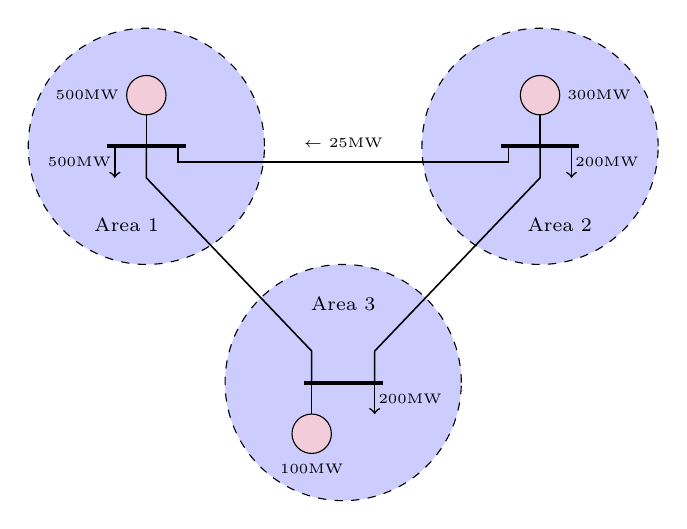
\begin{tikzpicture}
	
	% Area 1
	\draw [dashed, fill=blue!20] (0.5,0) circle (1.5cm);
		
	% Area 2
	\draw [dashed, fill=blue!20] (5.5,0) circle (1.5cm);
	
	% Area 3
	\draw [dashed, fill=blue!20] (3,-3) circle (1.5cm);
	
	% Area labels
	\node at (0.25,-1) {\scriptsize Area 1};
	\node at (5.75,-1) {\scriptsize Area 2};
	\node at (3,-2) {\scriptsize Area 3};
	
	% Bus 1
	\draw [line width=0.5mm] (0,0) -- (1,0);
	\draw [line width=0.2mm] (0.5,0) -- (0.5,0.4);
	
	% Load 1
	\draw [->, line width=0.2mm] (0.1,0) -- (0.1,-0.4);
	\node at (-0.35,-0.2) {\tiny 500MW};
	
	% Gen 1
	\draw [fill=purple!20] (0.5,0.65) circle (0.25cm);
	\node at (-0.25,0.65) {\tiny 500MW};
	
	% Bus 2
	\draw [line width=0.5mm] (5,0) -- (6,0);
	\draw [line width=0.2mm] (5.5,0) -- (5.5,0.4);
	
	% Load 2
	\draw [->, line width=0.2mm] (5.9,0) -- (5.9,-0.4);
	\node at (6.35,-0.2) {\tiny 200MW};
	
	% Gen 2
	\draw [fill=purple!20] (5.5,0.65) circle (0.25cm);
	\node at (6.25,0.65) {\tiny 300MW};
	
	% Bus 3
	\draw [line width=0.5mm] (2.5,-3) -- (3.5,-3);
	\draw [line width=0.2mm] (2.6,-3) -- (2.6,-3.4);
	
	% Load 3
	\draw [->, line width=0.2mm] (3.4,-3) -- (3.4,-3.4);
	\node at (3.85,-3.2) {\tiny 200MW};
	
	% Gen 3
	\draw [fill=purple!20] (2.6,-3.65) circle (0.25cm);
	\node at (2.6,-4.1) {\tiny 100MW};
	
	% Tie line 1 to 2
	\draw [line width=0.2mm] (0.9,0) -- (0.9,-0.2) -- (5.1,-0.2) -- (5.1,0);
	
	% Tie line 1 to 3
	\draw [line width=0.2mm] (0.5,0) -- (0.5,-0.4) -- (2.6,-2.6) -- (2.6,-3);
	
	% Tie line 2 to 3
	\draw [line width=0.2mm] (5.5,0) -- (5.5,-0.4) -- (3.4,-2.6) -- (3.4,-3);
	
	% Flow from 2 to 1
	\node at (3, 0.05) {\tiny $\leftarrow$ 25MW};
	
	% Flow from 1 to 3
	
	
	% Flow from 3 to 2
	
	
	
\end{tikzpicture}}
	\caption[Multiple area power system]{An example of three interconnected control areas in a 60$\si{\hertz}$ power system. The interconnections allow power to flow from one area to another, allowing generators to service loads from different areas. Each control area consists of several generators and loads, but are modelled with a single generator and single load for simplicity \cite{Grainger1994}.}
	\label{fig:2105_multiple_area_system}
\end{figure}

Typically, for each control area, many loads will be aggregated into a single load, and many generators into a single generator, in order to simplify the model \cite{Grainger1994}. The simplest power system to control is one that consists of a single control area. A single control area power system has no interconnections to any other control area. It is comprised of a consumer load demand, and a set of generators, some of which are acting as regulating units. As previously mentioned, for modelling simplicity, loads are aggregated to a single load, and generators can be aggregated to a single generator. This simple system, shown in Figure \ref{fig:2106_single_area_system_overview} is well understood.

\begin{figure}[h]
	\centering
	\resizebox{4.5cm}{!}{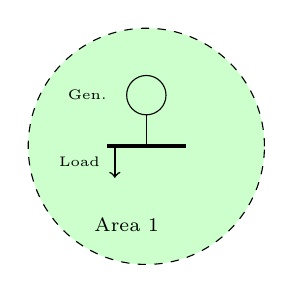
\begin{tikzpicture}
	
	% Area 1
	\draw [dashed, fill=white!80!green] (0.5,0) circle (1.5cm);

	% Area labels
	\node at (0.25,-1) {\scriptsize Area 1};
	
	% Bus 1
	\draw [line width=0.5mm] (0,0) -- (1,0);
	\draw [line width=0.2mm] (0.5,0) -- (0.5,0.4);
	
	% Load 1
	\draw [->, line width=0.2mm] (0.1,0) -- (0.1,-0.4);
	\node at (-0.35,-0.2) {\tiny Load};
	
	% Gen 1
	\draw (0.5,0.65) circle (0.25cm);
	\node at (-0.25,0.65) {\tiny Gen.};

\end{tikzpicture}
}
	\caption[Single area power system]{A single area power system has a load and a generator, with no connections to other power areas}
	\label{fig:2106_single_area_system_overview}
\end{figure}

When expressing the single area model mathematically, researchers consider three separate elements: the governor, the turbine, and the generator-load.

\subsubsection{Governor Model} \label{sec:governor_model}
The governor is a device which is used to regulate the speed of a generator. It is often modelled as a first order system, as shown in Figure \ref{fig:2107_governor_model}. The governor receives an input, $\Delta P_C(s)$, which represents a power increase/decrease command brought about by adjusting the governor speed changer. Older governors operated by mechanically coupling the governor with the rotating shaft of the generator; however, newer governors operate electronically. Owing to the older mechanical governor designs, governor models often include a proportional feedback loop using turbine rotational frequency change, $\Delta F(s)$. The output, $\Delta Y_E(s)$, represents a control signal to change the turbine steam valve position. The model parameter $K_{sg}$ is the static gain of the speed-governing mechanism, and the parameter $T_{sg}$ is the time constant of the speed-governing mechanism.

The frequency domain derivation of the governor model can be found in Appendix \ref{app:governor_model}.

\begin{figure}[h]
	\centering
	\begin{tikzpicture}

\end{tikzpicture}
	\caption[Frequency domain model for governor]{Frequency domain model for the generator governor.}
	\label{fig:2107_governor_model}
\end{figure}

\subsubsection{Turbine Model}
A steam turbine converts energy stored in the form of high pressure and high temperature steam into rotational energy. The steam is created in a boiler heated by fossil fuel combustion. Alternatively, a nuclear reactor could be used to produce the heat. As the steam is forced through turbine nozzle sections it is accelerated to high velocities. Kinetic energy from the high velocity steam is converted into shaft torque as it collides with moving blades attached to the turbine rotor. Coupling the turbine rotor to a synchronous machine converts rotational energy to electrical energy.

Steam turbines can come in a variety of configurations with multiple turbines, and steam reheating systems being common features in modern machinery. The model presented in this section has omitted many of these details, providing a simpler representation. The model, shown in Figure \ref{fig:2108_turbine_model}, is a first-order system that takes the input $\Delta Y_E(s)$, representing the change in steam valve position. The model output is denoted as $\Delta P_G(s)$, which represents the change in power output of the turbine. An increase in the $\Delta Y_E(s)$ lets additional steam into the turbine, increasing $\Delta P_G(s)$. Conversely, a decrease in $\Delta Y_E()$, restricts the steam inflow, reducing $\Delta P_G(s)$.

The frequency domain derivation of the governor model can be found in Appendix \ref{app:turbine_model}.

\begin{figure}[h]
	\centering
	% Set up the standalone document class
\documentclass{standalone}

% Input the preamble (<3)
% Preamble document

% Import tikz package
\usepackage{tikz}

% Import tikz libraries
\usetikzlibrary{shapes, arrows}
\usetikzlibrary{positioning, calc}

%----------- Create a fancy summing block
\tikzset{add/.style n args={4}{
		minimum width=6mm,
		path picture={
			\draw[black] 
			(path picture bounding box.south east) -- (path picture bounding box.north west)
			(path picture bounding box.south west) -- (path picture bounding box.north east);
			\node at ($(path picture bounding box.south)+(0,0.13)$)     {\tiny #1};
			\node at ($(path picture bounding box.west)+(0.13,0)$)      {\tiny #2};
			\node at ($(path picture bounding box.north)+(0,-0.13)$)    {\tiny #3};
			\node at ($(path picture bounding box.east)+(-0.13,0)$)     {\tiny #4};
		}
	}
}

%----------- Block style 1
\tikzstyle{block1} = [draw, fill=blue!20, rectangle, 
minimum height=3em, minimum width=6em, node distance=2.5cm]

%----------- Block style 2
\tikzstyle{block2} = [draw, fill=blue!20, rectangle, 
minimum height=3em, minimum width=3em, node distance=2.5cm]

%----------- Sum style
\tikzstyle{sum} = [draw, fill=blue!20, circle, node distance=2cm]

%----------- Input style
\tikzstyle{input} = [coordinate, node distance=4cm]

%----------- Output style
\tikzstyle{output} = [coordinate, node distance=4cm]

%----------- Pin style
\tikzstyle{pinstyle} = [pin edge={to-,thin,black}]

\begin{document}

\begin{tikzpicture}

	% Draw the nodes first
	\node [input] (input) {};
	\node [block1, right of=input, node distance=4cm, label=above:{Turbine}] (turbine) {$\frac{K_{t}}{1 + T_{t}s}$};
	\node [output, right of=turbine] (output) {};
	
	% Connect the nodes
	\draw [->] (input) -- node [label=above:{$\Delta Y_E(s)$}] {} (turbine);
	\draw [->] (turbine) -- node [label=above:{$\Delta P_G(s)$}] {} (output);
	
\end{tikzpicture}

\end{document}
	\caption[Frequency domain model for governor]{Frequency domain model for the generator turbine.}
	\label{fig:2108_turbine_model}
\end{figure}

\subsubsection{Generator Load Model}
Consumers connected to the power system change their demand for power as appliances are switched on and off, placing demand on the generator. The incremental power demanded by consumers, $\Delta P_L(s)$, is subtracted from the incremental power delivered by the turbine to form the input for the generator-load model. The model, shown in Figure \ref{fig:2109_generator_load_model}, is first-order and change in frequency as the output, denoted by $\Delta F(s)$. As the incremental power demanded increases, the generator frequency decreases. Conversely, as the incremental power demanded decreases, the generator frequency increases.

The frequency domain derivation of the governor model can be found in Appendix \ref{app:gen_load_model}.

\begin{figure}[h]
	\centering
	% Set up the standalone document class
\documentclass{standalone}

% Input the preamble (<3)
% Preamble document

% Import tikz package
\usepackage{tikz}

% Import tikz libraries
\usetikzlibrary{shapes, arrows}
\usetikzlibrary{positioning, calc}

%----------- Create a fancy summing block
\tikzset{add/.style n args={4}{
		minimum width=6mm,
		path picture={
			\draw[black] 
			(path picture bounding box.south east) -- (path picture bounding box.north west)
			(path picture bounding box.south west) -- (path picture bounding box.north east);
			\node at ($(path picture bounding box.south)+(0,0.13)$)     {\tiny #1};
			\node at ($(path picture bounding box.west)+(0.13,0)$)      {\tiny #2};
			\node at ($(path picture bounding box.north)+(0,-0.13)$)    {\tiny #3};
			\node at ($(path picture bounding box.east)+(-0.13,0)$)     {\tiny #4};
		}
	}
}

%----------- Block style 1
\tikzstyle{block1} = [draw, fill=blue!20, rectangle, 
minimum height=3em, minimum width=6em, node distance=2.5cm]

%----------- Block style 2
\tikzstyle{block2} = [draw, fill=blue!20, rectangle, 
minimum height=3em, minimum width=3em, node distance=2.5cm]

%----------- Sum style
\tikzstyle{sum} = [draw, fill=blue!20, circle, node distance=2cm]

%----------- Input style
\tikzstyle{input} = [coordinate, node distance=4cm]

%----------- Output style
\tikzstyle{output} = [coordinate, node distance=4cm]

%----------- Pin style
\tikzstyle{pinstyle} = [pin edge={to-,thin,black}]

\begin{document}

\begin{tikzpicture}
	
	% Draw the nodes first
\end{tikzpicture}

\end{document}
	\caption[Frequency domain model for generator-load]{Frequency domain model for the generator-load.}
	\label{fig:2109_generator_load_model}
\end{figure}


%------------------------ SS: Single Area

\subsection{Frequency Control for a Single Area System}\label{sec:control_one_area_system}
It is common for a speed droop governor feedback control regime to perform primary frequency control, with an AGC feedback loop used to perform secondary frequency control when restoring a minor frequency excursion \cite{Wood2013, Grainger1994, Kothari2011, Kundur1994}. A particularly well laid out approach to developing linear models for the turbine, generator, load, and governor was presented by Kundur \cite{Kundur1994}. The full model is shown in Figure \ref{fig:2110_single_area_pi_control_model}. This model is described by a single regulating generator supplying a load. The governor block is a first-order linear model of the governor. The turbine block is a first-order linear model of the turbine. The final block is the generator-load, which is also a first-order linear model. The AGC feedback loop uses a proportional integral controller.

\clearpage

\begin{sidewaysfigure}[ht]
\centering
% Set up the standalone document class
\documentclass{standalone}

% Input the preamble (<3)
% Preamble document

% Import tikz package
\usepackage{tikz}

% Import tikz libraries
\usetikzlibrary{shapes, arrows}
\usetikzlibrary{positioning, calc}

%----------- Create a fancy summing block
\tikzset{add/.style n args={4}{
		minimum width=6mm,
		path picture={
			\draw[black] 
			(path picture bounding box.south east) -- (path picture bounding box.north west)
			(path picture bounding box.south west) -- (path picture bounding box.north east);
			\node at ($(path picture bounding box.south)+(0,0.13)$)     {\tiny #1};
			\node at ($(path picture bounding box.west)+(0.13,0)$)      {\tiny #2};
			\node at ($(path picture bounding box.north)+(0,-0.13)$)    {\tiny #3};
			\node at ($(path picture bounding box.east)+(-0.13,0)$)     {\tiny #4};
		}
	}
}

%----------- Block style 1
\tikzstyle{block1} = [draw, fill=blue!20, rectangle, 
minimum height=3em, minimum width=6em, node distance=2.5cm]

%----------- Block style 2
\tikzstyle{block2} = [draw, fill=blue!20, rectangle, 
minimum height=3em, minimum width=3em, node distance=2.5cm]

%----------- Sum style
\tikzstyle{sum} = [draw, fill=blue!20, circle, node distance=2cm]

%----------- Input style
\tikzstyle{input} = [coordinate, node distance=4cm]

%----------- Output style
\tikzstyle{output} = [coordinate, node distance=4cm]

%----------- Pin style
\tikzstyle{pinstyle} = [pin edge={to-,thin,black}]

\begin{document}
	
\begin{tikzpicture}
	
	% Draw the nodes first
	\node [input] (input) {};
	\node [block2, right of=input] (integral) {$\frac{K_i}{s}$};
	\node [sum, add={$-$}{+}{ }{ }, right of=integral, node distance=2.5cm] (sum1) {};
	\node [block1, right of=sum1, label=above:{Governor}] (governor) {$\frac{K_{sg}}{1 + T_{sg}s}$};
	\node [block2, below of=governor] (regulator) {$\frac{1}{R}$};
	\node [coordinate, below of=regulator] (feedback2) {};
	\node [block1, right of=governor, label=above:{Turbine}, node distance=4cm] (turbine) {$\frac{K_t}{1 + T_t s}$};
	\node [sum, add={ }{+}{$-$}{ }, right of=turbine, node distance=3cm] (sum2) {};
	\node [input, above of=sum2, node distance=2cm] (demand) {};
	\node [block1, right of=sum2, label=above:{Gen. Load}] (genload) {$\frac{K_{gl}}{1 + T_{gl}s}$};
	\node [output, right of=genload] (output) {};
	
	% Connect the nodes
	\draw [->] (input) -- (integral);
	\draw [->] (integral) -- node [label=above:{$\Delta P_C(s)$}] {} (sum1);
	\draw [->] (sum1) -- (governor);
	\draw [->] (governor) -- node [label=above:{$\Delta Y_E(s)$}] {} (turbine);
	\draw [->] (turbine) -- node [label=above:{$\Delta P_G(s)$}] {} (sum2);
	\draw [->] (demand) -- node [label=right:{$\Delta P_L(s)$}] {} (sum2);
	\draw [->] (sum2) -- (genload);
	\draw [->] (genload) -- node [coordinate, name=feedback1, label=above:{$\Delta F(s)$}] {} (output);
	\draw [->] (feedback1) |- (regulator);
	\draw [->] (regulator) -| (sum1);
	\draw (feedback1) |- (feedback2);
	\draw (feedback2) -| (input);
	
\end{tikzpicture}

\end{document}
\caption[Single power area with PI feedback control]{A classical feedback control approach for a single control area power system. The system is comprised of a first order models for both turbines, and generators. The governor controllers are also first order models. AGC is implemented using an integral control block in a feedback loop \cite{Kundur1994}.}
\label{fig:2110_single_area_pi_control_model}
\end{sidewaysfigure}

\clearpage

%------------------------ SS: Modelling a Two Area System

\subsection{Modelling a Two Area System} \label{ssec:modelling_two_area_system}
The single area system presented in Section \ref{sec:modelling_a_single_area} is useful to help understand the role of governors and AGC in controlling power system frequency. In reality, power systems are comprised of many control areas connected by transmission lines, referred to as tie lines. Often, there is some net power transfer over the tie lines, dictated by contractual agreement. Single area models do not describe this additional complexity. The simplest model that includes tie lines is the two area power system, shown in Figure \ref{fig:2111_two_area_system}.

\begin{figure}[h]
	\centering
	\resizebox{12cm}{!}{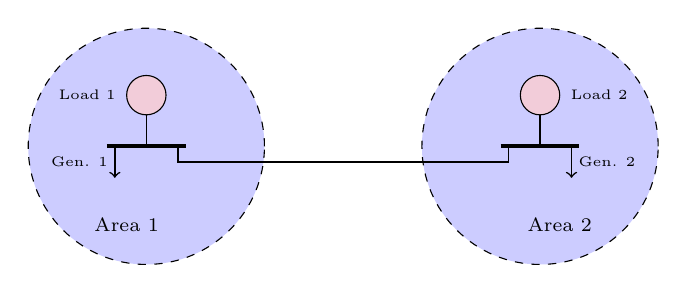
\begin{tikzpicture}
	
	% Area 1
	\draw [dashed, fill=blue!20] (0.5,0) circle (1.5cm);
		
	% Area 2
	\draw [dashed, fill=blue!20] (5.5,0) circle (1.5cm);
	
	% Area labels
	\node at (0.25,-1) {\scriptsize Area 1};
	\node at (5.75,-1) {\scriptsize Area 2};
	
	% Bus 1
	\draw [line width=0.5mm] (0,0) -- (1,0);
	\draw [line width=0.2mm] (0.5,0) -- (0.5,0.4);
	
	% Load 1
	\draw [->, line width=0.2mm] (0.1,0) -- (0.1,-0.4);
	\node at (-0.35,-0.2) {\tiny Gen. 1};
	
	% Gen 1
	\draw [fill=purple!20] (0.5,0.65) circle (0.25cm);
	\node at (-0.25,0.65) {\tiny Load 1};
	
	% Bus 2
	\draw [line width=0.5mm] (5,0) -- (6,0);
	\draw [line width=0.2mm] (5.5,0) -- (5.5,0.4);
	
	% Load 2
	\draw [->, line width=0.2mm] (5.9,0) -- (5.9,-0.4);
	\node at (6.35,-0.2) {\tiny Gen. 2};
	
	% Gen 2
	\draw [fill=purple!20] (5.5,0.65) circle (0.25cm);
	\node at (6.25,0.65) {\tiny Load 2};
	
	% Tie line 1 to 2
	\draw [line width=0.2mm] (0.9,0) -- (0.9,-0.2) -- (5.1,-0.2) -- (5.1,0);

\end{tikzpicture}
}
	\caption[Overview of two area power system with tie line]{A two area power system comprised of generators and load connected via a tie line. Power flows from one area to the other depending on the power demands.}
	\label{fig:2111_two_area_system}
\end{figure}

Governor, and turbine models presented in \textsection \ref{sec:modlling_a_single_area} are used in each of the power areas for a two-area power system model. Additionally, a model for the tie-line connection between the two power areas is used, as well as an updated generator-load model. 

\subsubsection{Tie Line Model}\label{sec:tie_line_model}
The transmission line connecting two power areas exports power from one area to another, allowing an increase or decrease in the input to the generator-load model for each area. This effect is implemented using a feedback loop. Inputs to the tie-line model are derived from frequency outputs from both areas. The values are differenced and converted to a change in power by multiplying by $2\pi$ and integrating the result. Outputs, $\Delta P_{tie,1}$ and $\Delta_{tie,2}$, represent incremental power supplied or received over the tie-line. The tie-line model is shown in Figure \ref{fig:2112_tie_line_model}. The model derivation can be found in Appendix \ref{fig:tie_line_model}.

\begin{figure}[h]
	\centering
	%----------- Create a fancy summing block
\tikzset{add/.style n args={4}{
		minimum width=6mm,
		path picture={
			\draw[black] 
			(path picture bounding box.south east) -- (path picture bounding box.north west)
			(path picture bounding box.south west) -- (path picture bounding box.north east);
			\node at ($(path picture bounding box.south)+(0,0.13)$)     {\tiny #1};
			\node at ($(path picture bounding box.west)+(0.13,0)$)      {\tiny #2};
			\node at ($(path picture bounding box.north)+(0,-0.13)$)    {\tiny #3};
			\node at ($(path picture bounding box.east)+(-0.13,0)$)     {\tiny #4};
		}
	}
}

%----------- Block style 1
\tikzstyle{block1} = [draw, fill=green!20, rectangle, 
minimum height=3em, minimum width=6em, node distance=2.5cm]

%----------- Block style 2
\tikzstyle{block2} = [draw, fill=green!20, rectangle, 
minimum height=3em, minimum width=3em, node distance=2.5cm]

%----------- Sum style
\tikzstyle{sum} = [draw, fill=green!20, circle, node distance=2cm]

%----------- Input style
\tikzstyle{input} = [coordinate, node distance=4cm]

%----------- Output style
\tikzstyle{output} = [coordinate, node distance=4cm]

\begin{tikzpicture}
	
	% Draw the nodes first
	\node [input] (input1) {};
	\node [sum,add={ }{+}{ }{$-$}, right of=input1, node distance=4cm] (sum) {};
	\node [right of=sum, node distance=6.55cm] (input2) {};
	\node [block1, above of=sum] (tieline) {$\frac{2 \pi T_{12}}{s}$};
	\node [block2, right of=tieline] (a12) {$-a_{12}$};
	\node [output, right of=a12] (P2) {};
	\node [output, left of=tieline] (P1) {};
	
	% Connect the nodes
	\draw [->] (input1) -- node [label=above:{$\Delta F_1(s)$}] {} (sum);
	\draw [->] (input2) -- node [label=above:{$\Delta F_2(s)$}] {} (sum);
	\draw [->] (sum) -- (tieline);
	\draw [->] (tieline) -- node[label=above:{$\Delta P_{tie,1}$}] {} (P1);
	\draw [->] (tieline) -- (a12);
	\draw [->] (a12) -- node[label=above:{$\Delta P_{tie,2}$}] {} (P2);
\end{tikzpicture}
	\caption[Frequency domain model for a transmission line]{Frequency domain model for the transmission line between two power areas.}
	\label{fig:2112_tie_line_model}
\end{figure}

\subsubsection{Generator Load Model for Two-Area Power System}
As mentioned in \textsection \ref{sec:tie_line_model}, the generator-load model either supplies or receives power via the tie-line connection between the two areas. To accommodate for this a feedback loop is implemented, which adds tie-line power back into the generator-load, as shown in Figure \ref{fig:2113_generator_load_model_1_with_tie_line}.

\begin{figure}[h]
	\centering
	%----------- Create a fancy summing block
\tikzset{add/.style n args={4}{
		minimum width=6mm,
		path picture={
			\draw[black] 
			(path picture bounding box.south east) -- (path picture bounding box.north west)
			(path picture bounding box.south west) -- (path picture bounding box.north east);
			\node at ($(path picture bounding box.south)+(0,0.13)$)     {\tiny #1};
			\node at ($(path picture bounding box.west)+(0.13,0)$)      {\tiny #2};
			\node at ($(path picture bounding box.north)+(0,-0.13)$)    {\tiny #3};
			\node at ($(path picture bounding box.east)+(-0.13,0)$)     {\tiny #4};
		}
	}
}

%----------- Block style 1
\tikzstyle{block1} = [draw, fill=green!20, rectangle, 
minimum height=3em, minimum width=6em, node distance=2.5cm]

%----------- Block style 2
\tikzstyle{block2} = [draw, fill=green!20, rectangle, 
minimum height=3em, minimum width=3em, node distance=2.5cm]

%----------- Sum style
\tikzstyle{sum} = [draw, fill=green!20, circle, node distance=2cm]

%----------- Input style
\tikzstyle{input} = [coordinate, node distance=4cm]

%----------- Output style
\tikzstyle{output} = [coordinate, node distance=4cm]

\begin{tikzpicture}
	
	% Draw the nodes first
	\node [input] (input) {};
	\node [sum,add={$-$}{+}{$-$}{ },right of=input] (sum) {};
	\node [block1, right of=sum, label=above:{Gen. Load}] (genload) {$\frac{K_{gl}}{1 + T_{gl}s}$};
	\node [input, above of=sum, node distance=2cm] (tieline) {};
	\node [input, below of=sum, node distance=2cm] (powerdemand) {};
	\node [output, right of=genload] (output) {};
	
	% Connect the nodes
	\draw [->] (input) -- node [label=above:{$\Delta P_G(s)$}] {} (sum);
	\draw [->] (sum) -- (genload);
	\draw [->] (powerdemand) -- node [label=right:{$\Delta P_{L, 1}(s)$}] {} (sum);
	\draw [->] (tieline) -- node [label=right:{$\Delta P_{tie, 1}$}] {} (sum);
	\draw [->] (genload) -- node [label=above:{$\Delta F(s)$}] {} (output);
	
\end{tikzpicture}
	\caption[Frequency domain model for generator-load with tie-line connection]{Frequency domain model for the generator-load with feedback from a tie-line.}
	\label{fig:2113_generator_load_model_1_with_tie_line}
\end{figure}

The frequency domain derivation of the generator-load model for a two area power system can be found in Appendix \ref{app:generator_load_model_with_tie_line}.

%------------------------ SS: Two Area

\subsection{Frequency Control for Two Area System} \label{ssec:control_two_area_system}
The control objective for a two area power system is to maintain the inter-area power transfer, whilst regulating the frequency of each area. An AGC integral feedback loop on regulating units, like that shown in Figure \ref{fig:2110_single_area_pi_control_model}, would ensure that power system frequency is maintained, however, would not guarantee inter-area power transfer agreements are observed.

Violation of power transfer contracts due to control issues does not allow for a stable market in which energy can be reliably traded. Fortunately, multi control area power systems are well understood, and classical control approaches have been successfully implemented to meet the new control objectives. In order to apply classical PI controllers to two-area power system control, a metric called Area Control Error (ACE) is used in the AGC feedback loop for each control area. ACE is a linear combination of the frequency deviations and tie-line power flows.

The two-area power system can be modelled using governor, turbine, tie-line and generator-load models developed in \textsection \ref{sec:modelling_a_single_area} and \textsection \ref{ssec:control_two_area_system}. This is shown shown in Figure \ref{fig:208_two_area_pi_control_model}, in addition to the classical PI controller with ACE input.

\clearpage

\begin{sidewaysfigure}[ht]
\centering
\resizebox{22cm}{!}{%----------- Create a fancy summing block
\tikzset{add/.style n args={4}{
		minimum width=6mm,
		path picture={
			\draw[black] 
			(path picture bounding box.south east) -- (path picture bounding box.north west)
			(path picture bounding box.south west) -- (path picture bounding box.north east);
			\node at ($(path picture bounding box.south)+(0,0.13)$)     {\tiny #1};
			\node at ($(path picture bounding box.west)+(0.13,0)$)      {\tiny #2};
			\node at ($(path picture bounding box.north)+(0,-0.13)$)    {\tiny #3};
			\node at ($(path picture bounding box.east)+(-0.13,0)$)     {\tiny #4};
		}
	}
}

%----------- Block style 1
\tikzstyle{block1} = [draw, fill=white!80!green, rectangle, 
minimum height=3em, minimum width=6em, node distance=2.5cm]

%----------- Block style 2
\tikzstyle{block2} = [draw, fill=white!80!blue, rectangle, 
minimum height=3em, minimum width=3em, node distance=2.5cm]

%----------- Sum style
\tikzstyle{sum} = [draw, fill=white!80!green, circle, node distance=2cm]

%----------- Input style
\tikzstyle{input} = [coordinate, node distance=4cm]

%----------- Output style
\tikzstyle{output} = [coordinate, node distance=4cm]

%----------- Pin style
\tikzstyle{pinstyle} = [pin edge={to-,thin,black}]

\begin{tikzpicture}	
	% Tie line nodes
	\node [sum, add={$-$}{}{+}{ }] (sum1) {};
	\node [block1, right of=sum1, label=above:{Tie Line}] (tieline) {$\frac{2\pi T_{12}}{s}$};
	\node [output, right of=tieline, node distance=2cm] (out) {};
	\node [coordinate, above of=out, node distance=5cm] (c1) {};
	\node [coordinate, below of=out, node distance=5cm] (c2) {};
	\node [block2, left of=c2, fill=white!80!green] (a12) {$-a_{12}$};
	
	% Position a reference coordinate for drawing
	\node [coordinate, left of=sum1, node distance=2.5cm] (c3) {};
	\node [coordinate, above of=c3, node distance=0.75cm] (c4) {};
	\node [coordinate, below of=c3, node distance=0.75cm] (c5) {};
	
	% Create nodes for upper leg
	\node [block1, above of=c3, node distance=3.5cm, label=above:{Gen. Load 1}] (genload1) {$\frac{K_{gl1}}{T_{gl1}s+1}$};
	\node [coordinate, right of=genload1, node distance=1.5cm] (c6) {};
	\node [sum, left of=genload1, add={$-$}{+}{$-$}{}, node distance=2.5cm] (sum2) {};
	\node [coordinate, below of=sum2] (p11) {};
	\node [coordinate, left of=p11, node distance=0.5cm, label=left:{$\Delta P_{L1}(s)$}] (p12) {};
	\node [block1, left of=sum2, node distance=3.5cm, label=above:{Turbine 1}] (turbine1) {$\frac{K_{t1}}{T_{t1}s+1}$};
	\node [block1, left of=turbine1, node distance=4.5cm, label=above:{Governor 1}] (governor1) {$\frac{K_{g1}}{T_{g1}s+1}$};
	\node [sum, left of=governor1, add={$-$}{}{+}{}, node distance=2.5cm, fill=white!80!blue] (sum4) {};
	\node [block2, below of=sum4, node distance=1.75cm] (r1) {$R_1$};
	\node [block2, left of=sum4] (int1) {$\frac{K_{i2}}{s}$};
	\node [sum, left of=int1, add={+}{ }{+}{ }, fill=white!80!blue] (sum6) {};
	\node [block2, below of=sum6, node distance=1.75cm] (b1) {$b_1$};
	
	% Create nodes for lower leg
	\node [block1, below of=c3, node distance=3.5cm, label=above:{Gen. Load 2}] (genload2) {$\frac{K_{gl1}}{T_{gl1}s+1}$};
	\node [coordinate, right of=genload2, node distance=1.5cm] (c7) {};
	\node [sum, left of=genload2, add={$-$}{+}{$-$}{}, node distance=2.5cm] (sum3) {};
	\node [coordinate, above of=sum3] (p21) {};
	\node [coordinate, left of=p21, node distance=0.5cm, label=left:{$\Delta P_{L2}(s)$}] (p22) {};
	\node [block1, left of=sum3, node distance=3.5cm, label=above:{Turbine 2}] (turbine2) {$\frac{K_{t2}}{T_{t2}s+1}$};
	\node [block1, left of=turbine2, node distance=4.5cm, label=above:{Governor 2}] (governor2) {$\frac{K_{g2}}{T_{g2}s+1}$};
	\node [sum, left of=governor2, add={+}{}{$-$}{}, node distance=2.5cm, fill=white!80!blue] (sum5) {};
	\node [block2, above of=sum5, node distance=1.75cm] (r2) {$R_2$};
	\node [block2, left of=sum5] (int2) {$\frac{K_{i2}}{s}$};
	\node [sum, left of=int2, add={+}{ }{+}{ }, fill=white!80!blue] (sum7) {};
	\node [block2, above of=sum7, node distance=1.75cm] (b2) {$b_2$};
	
	
	
	% Connect the tieline nodes
	\draw [->] (sum1) -- (tieline);
	\draw (tieline) -- (out);
	
	% Connect nodes in upper block
	\draw (out) -- node [label=right:{$\Delta P_{tie,1}(s)$}] {} (c1);
	\draw [->] (c1) -| (sum2);
	\draw [->] (c1) -| (sum6);
	\draw [->] (sum4) -- (governor1);
	\draw [->] (governor1) -- node [label=above:{$\Delta Y_{E1}(s)$}] {} (turbine1);
	\draw [->] (turbine1) -- node [label=above:{$\Delta P_{G1}(s)$}] {} (sum2);
	\draw [->] (sum2) -- (genload1);
	\draw [->] (genload1) -| node [label=above:{$\Delta F_1(s)$}] {} (sum1);
	\draw (c6) |- (c4);
	\draw [->] (c4) -| (r1);
	\draw [->] (c4) -| (b1);
	\draw [->] (r1) -- (sum4);
	\draw (p12) -- (p11);
	\draw [->] (p11) -- (sum2);
	\draw [->] (sum6) -- (int1);
	\draw [->] (int1) -- (sum4);
	\draw [->] (b1) -- (sum6);
	
	% Connect nodes in lower block
	\draw (out) -- node [label=right:{$\Delta P_{tie,2}(s)$}] {} (c2);
	\draw [->] (c2) -- (a12);
	\draw [->] (a12) -| (sum3);
	\draw [->] (a12) -| (sum7);
	\draw [->] (sum5) -- (governor2);
	\draw [->] (governor2) -- node [label=below:{$\Delta Y_{E2}(s)$}] {} (turbine2);
	\draw [->] (turbine2) -- node [label=below:{$\Delta P_{G2}(s)$}] {} (sum3);
	\draw [->] (sum3) -- (genload2);
	\draw [->] (genload2) -| node [label=below:{$\Delta F_2(s)$}] {} (sum1);
	\draw (c7) |- (c5);
	\draw [->] (c5) -| (r2);
	\draw [->] (c5) -| (b2);
	\draw [->] (r2) -- (sum5);
	\draw (p22) -- (p21);
	\draw [->] (p21) -- (sum3);
	\draw [->] (sum7) -- (int2);
	\draw [->] (int2) -- (sum5);
	\draw [->] (b2) -- (sum7);
\end{tikzpicture}
}
\caption[Two area power system with PI feedback control]{A classical feedback control approach to a two area power system \cite{Kundur1994}.}
\label{fig:208_two_area_pi_control_model}
\end{sidewaysfigure}

\clearpage